\paragraph{Reibung}
\label{sec:physik:reibung}

Reibung ist ein faszinierendes Thema. Zum Einen stecken wir Menschen sehr viel Zeit in Entwicklungen um die Reibung zu vermindern, zum Anderen brauchen wir aber Reibung um überhaupt gehen zu können -- und manchmal ist es sogar notwendig, Zeit zu investieren um Reibung zu erhalten.

Eine der faszinierendsten Formen der Reibung ist die \textbf{Haftgleitreibung} (im Englischen: \emph{stick-slip motion}). Der Begriff Haftgleitreibung beschreibt den Effekt hervorragend: zwei Objekt wechseln zwischen \emph{Haften} und \emph{Gleiten}: Dies führt zu ruckartigen Bewegungen, die meistens nicht erwünscht sind -- in anderen Fällen aber gewünscht werden. Ein gutes Beispiel für die gewünschte Wirkung der Haftgleitreibung ist der Geigenbogen: obwohl man den Effekt nicht direkt wahrnimmt: er ist die Ursache dafür, dass die gestrichene Saite einen Ton erzeugt. Falls Ihr selbst ein Streichinstrument spielt oder einen Streicher beobachtet habt: um diese Haftgleitreibung des Bogens zu erhalten, ist es notwendig, den Bogen mit einem Harz (dem Kolophonium) regelmäßig einzustreichen. Die Haftgleitreibung ist übrigens auch dafür verantwortlich, dass die Kreide auf einer Kreidetafel quietscht. Falls Ihr gerne Computer-Spiele spielt, wird Euch überraschenderweise dieser Effekt da auch begegnen: die Minecraft-Gamer unter Euch nennen das ``Butterfly Clicking''. Dabei rutscht der Klick-Finger so über die Maustaste, dass man mit er Maustaste hohe Klick-Raten erzeugt. 
% TODO: Reihenfolge der Beispiele überdenken (Minecraft zuerst, dann Geige/Kreide).
% TODO: "Butterfly Clicking" kurz erklären (Stick-Slip: kurz haften, dann rutschen).
% TODO: Fußnote/Box: Verweis auf Resonanz (Geige) als "später mehr" markieren.
% TODO: Klimax/Übergang schärfen: Von der Alltagsreibung zurück zum Sandkorn/Luftwiderstand (Brücke zur Regensimulation).

Die Art von Reibung die Euch selbst jeden Tag begenet ist die \textbf{Gleitreibung}. Die ist Euch bestimmt schon mal beim Schlittschuhlaufen begegnet: nachdem Ihr Euch abgestoßen habt, werdet Ihr langsamer. Es fühlt sich so an, egal wie kräftig Ihr Euch abstoßt, als ob jemand auf der Bremse steht -- egal wie schell, immer das gleiche Langsamerwerden. In der Tat spielt auch Haftung wieder eine Rolle, denn zum Abstoßen braucht Ihr mehr Kraft. Aber sobald Ihr Euch bewegt, hängt die Reibung nur von Eurem Gewicht\footnote{%
    Habt Ihr Euch schonmal Gedanken gemacht, was eine Waage eigentlich misst? Die Waage, die Ihr aus dem Badezimmer kennt ist eine sogenannte Federwaage. Sie misst die Kraft, mit der Ihr auf die Erde angezogen werdet. Omas Küchenwaage jedoch, solche, wo Ihr vorne eine ein ``Gewicht'' verschiebt, vergleicht Gewichte -- hier wird tatsächlich die Masse ermittelt. Diese Technik wird schon seit vielen Jahrhunderten benutzt: dabei werden zwei Teller an einen Stab gehängt, der in der Mitte aufgehangen wird. Wenn beide Teller sich ``die Waage halten'' sind die Gewichte (Massen) auf beiden Seiten gleich. Diese Art von Waagen würden auf dem Mond genau gleich funktionieren, während die Federwaage nur ein Sechstel des Gewichts anzeigen würde.}
ab. Die Ursache dafür hängt damit zusammen, wie Oberflächen sich miteinander ``verzahnen''. Aber es gibt ``Gegenmaßnahmen''. In mechanischen Geräten benutzt man zum Beispiel Öl, dass diese Verzahnung erschwert -- die Bauteile gleiten dadurch leichter aneinander. Beim Schlittschuhfahren ist es das Wasser, dass die Reibung vermindert. ``Das Wasser?'' werden Ihr jetzt fragen -- ja, in der Tat hat die Form Eurer Kufen damit etwas zu tun: an der Spitze der Kufe ist der Druck so groß, dass das Eis wieder flüssig wird: man gleitet auf einer Wasserschicht. 
% TODO: zu harter Übergang zum Thema Gleitreibung

% TODO: Rollreibung erwähnen oder nicht?

Was passiert jetzt aber nun mit einem Gegenstand -- dem Regentropfen, der zur Erde fällt. Der Gegenstand bewegt sich durch die Luft, und die steht ihm buchstäblich im Weg: Er muss die Luftmoleküle beiseiteschieben, und das bremst ihn ab. Man nennt das \textbf{Luftwiderstand}. 
    
Machen wir aber erst einen Schritt zurück und schauen, was passiert, wenn die Luft keine Rolle spielt. Schaut Euch mal das Video an, dass die NASA während der Apollo 15 auf dem Mond gemacht hat (siehe QR-Code).\footnote{%
    \qrcode[height=2cm]{https://nssdc.gsfc.nasa.gov/planetary/image/AS15_Ham_feath_drop.mp4}}
Hier lässt der Astronaut einen Hammer und eine Feder gleichzeitig fallen: sie fallen tatsächlich gleich schnell auf die Mondoberfläche. Mehr noch: sie verhalten sich genau so, wie Newton es in seinem zweiten Gesetz aufschrieb und wir durch Formeln im letzten Abschnitt beschrieben haben.

Wie schnell so ein Regentropfen nun tatsächlich fällt, hängt von vielen Dingen ab: Wie groß ist er? Welche hoch ist Temperatur und der Luftdruck?\footnote{%
    Vereinfacht kann man sagen, dass Temperatur und Druck die Dichte beeinflussen, also die Menge an Luftmolekülen pro Volumen.}
Natürlich spielt auch die Form des Tropfens eine Rolle -- und die wird sogar von durch die Luft beeinflusst. Eine exakte Vorhersage ist deshalb ziemlich kompliziert.\footnote{%
    Tatsächlich braucht man sehr starke Computer um so etwas zu berechnen. Daher nutzt man für Autos, Flugzeuge, Raketen -- ja sogar für Gebäude -- Windkanäle. In diesen lässt sich die Strömung der Luft bei verschiedenen Geschwindigkeiten sehr genau beobachten.}
Aber wir können eine sehr gute Abschätzung machen, wenn wir ein paar dieser Dinge einfach ignorieren -- und genau das schauen wir uns jetzt an.
% TODO: die Berechnungen sind eher komplex - könnte man irgendwie einbauen

In der sogenannten Strömungsmechanik (das ist ein Teilgebiet der Physik und des Ingenieurswesens) benutzt man die folgende Formel, um den Luftwiderstand zu berechnen:
\begin{equation}
    F_\textrm{w}(v) = \frac12 \cdot c_\mathrm{w} \cdot A \cdot \varrho \cdot v^2 \,.
\end{equation}
wobei die Variablen die folgende Bedeutung haben:
\begin{description}
    \item[$c_\mathrm{w}$]Der Luftwiderstandsbeiwert (``Windschnittigkeit''). 
    \item[$A$] Die Querschnittsfläche des Körpers senkrecht zur Strömung. 
    \item[$\varrho$] Die Dichte der Luft. 
    \item[$v$] Die Geschwindigkeit des Körpers relativ zur Luft. 
\end{description}
Der $c_\mathrm{w}$ wird Euch vielleicht schon mal in einer Autowerbung begegnet sein, wenn darüber gesprochen wurde, dass ein Sportwagen einen besoders niedrigen $c_\mathrm{w}$-Wert hat und deshalb sehr windschnittig ist. In diesem Zusammenhang ist Euch vielleicht auch aufgefallen, dass in der Formel die Querschnittlsfläche $A$ folgt: das ist der Grund warum Sportwagen so flach sind -- halbe Höhe bedeutet halber Luftwiderstand. Für die Dichte hat sich bei Berechnung ein Standardwert \qty{1,225}{\kg\per\meter^3} eingebürgert (das ist ungefähr die Dichte von Luft auf Meereshöhe bei \qty{15}{\degreeCelsius}). Als letzten Teil der Gleichung findet Ihr aber nun $v^2$ (errinert Euch an das erste Kapitel, wo wir die Potenzen angesprochen haben): das heißt, die Geschwindigkeit geht quadratisch ein -- doppelte Geschwindigkeit führt zum vierfachen Luftwiderstand.
\begin{figure}[h]
    % GNUPLOT: LaTeX picture with Postscript
\begingroup
  \makeatletter
  \providecommand\color[2][]{%
    \GenericError{(gnuplot) \space\space\space\@spaces}{%
      Package color not loaded in conjunction with
      terminal option `colourtext'%
    }{See the gnuplot documentation for explanation.%
    }{Either use 'blacktext' in gnuplot or load the package
      color.sty in LaTeX.}%
    \renewcommand\color[2][]{}%
  }%
  \providecommand\includegraphics[2][]{%
    \GenericError{(gnuplot) \space\space\space\@spaces}{%
      Package graphicx or graphics not loaded%
    }{See the gnuplot documentation for explanation.%
    }{The gnuplot epslatex terminal needs graphicx.sty or graphics.sty.}%
    \renewcommand\includegraphics[2][]{}%
  }%
  \providecommand\rotatebox[2]{#2}%
  \@ifundefined{ifGPcolor}{%
    \newif\ifGPcolor
    \GPcolortrue
  }{}%
  \@ifundefined{ifGPblacktext}{%
    \newif\ifGPblacktext
    \GPblacktexttrue
  }{}%
  % define a \g@addto@macro without @ in the name:
  \let\gplgaddtomacro\g@addto@macro
  % define empty templates for all commands taking text:
  \gdef\gplbacktext{}%
  \gdef\gplfronttext{}%
  \makeatother
  \ifGPblacktext
    % no textcolor at all
    \def\colorrgb#1{}%
    \def\colorgray#1{}%
  \else
    % gray or color?
    \ifGPcolor
      \def\colorrgb#1{\color[rgb]{#1}}%
      \def\colorgray#1{\color[gray]{#1}}%
      \expandafter\def\csname LTw\endcsname{\color{white}}%
      \expandafter\def\csname LTb\endcsname{\color{black}}%
      \expandafter\def\csname LTa\endcsname{\color{black}}%
      \expandafter\def\csname LT0\endcsname{\color[rgb]{1,0,0}}%
      \expandafter\def\csname LT1\endcsname{\color[rgb]{0,1,0}}%
      \expandafter\def\csname LT2\endcsname{\color[rgb]{0,0,1}}%
      \expandafter\def\csname LT3\endcsname{\color[rgb]{1,0,1}}%
      \expandafter\def\csname LT4\endcsname{\color[rgb]{0,1,1}}%
      \expandafter\def\csname LT5\endcsname{\color[rgb]{1,1,0}}%
      \expandafter\def\csname LT6\endcsname{\color[rgb]{0,0,0}}%
      \expandafter\def\csname LT7\endcsname{\color[rgb]{1,0.3,0}}%
      \expandafter\def\csname LT8\endcsname{\color[rgb]{0.5,0.5,0.5}}%
    \else
      % gray
      \def\colorrgb#1{\color{black}}%
      \def\colorgray#1{\color[gray]{#1}}%
      \expandafter\def\csname LTw\endcsname{\color{white}}%
      \expandafter\def\csname LTb\endcsname{\color{black}}%
      \expandafter\def\csname LTa\endcsname{\color{black}}%
      \expandafter\def\csname LT0\endcsname{\color{black}}%
      \expandafter\def\csname LT1\endcsname{\color{black}}%
      \expandafter\def\csname LT2\endcsname{\color{black}}%
      \expandafter\def\csname LT3\endcsname{\color{black}}%
      \expandafter\def\csname LT4\endcsname{\color{black}}%
      \expandafter\def\csname LT5\endcsname{\color{black}}%
      \expandafter\def\csname LT6\endcsname{\color{black}}%
      \expandafter\def\csname LT7\endcsname{\color{black}}%
      \expandafter\def\csname LT8\endcsname{\color{black}}%
    \fi
  \fi
    \setlength{\unitlength}{0.0500bp}%
    \ifx\gptboxheight\undefined%
      \newlength{\gptboxheight}%
      \newlength{\gptboxwidth}%
      \newsavebox{\gptboxtext}%
    \fi%
    \setlength{\fboxrule}{0.5pt}%
    \setlength{\fboxsep}{1pt}%
    \definecolor{tbcol}{rgb}{1,1,1}%
\begin{picture}(6800.00,4520.00)%
    \gplgaddtomacro\gplbacktext{%
      \csname LTb\endcsname%%
      \put(538,697){\makebox(0,0)[r]{\strut{}$0$}}%
      \csname LTb\endcsname%%
      \put(538,1593){\makebox(0,0)[r]{\strut{}$5$}}%
      \csname LTb\endcsname%%
      \put(538,2489){\makebox(0,0)[r]{\strut{}$10$}}%
      \csname LTb\endcsname%%
      \put(538,3385){\makebox(0,0)[r]{\strut{}$15$}}%
      \csname LTb\endcsname%%
      \put(538,4282){\makebox(0,0)[r]{\strut{}$20$}}%
      \csname LTb\endcsname%%
      \put(629,479){\makebox(0,0){\strut{}$0$}}%
      \csname LTb\endcsname%%
      \put(1804,479){\makebox(0,0){\strut{}$2$}}%
      \csname LTb\endcsname%%
      \put(2979,479){\makebox(0,0){\strut{}$4$}}%
      \csname LTb\endcsname%%
      \put(4155,479){\makebox(0,0){\strut{}$6$}}%
      \csname LTb\endcsname%%
      \put(5330,479){\makebox(0,0){\strut{}$8$}}%
      \csname LTb\endcsname%%
      \put(6505,479){\makebox(0,0){\strut{}$10$}}%
    }%
    \gplgaddtomacro\gplfronttext{%
      \csname LTb\endcsname%%
      \put(2734,4085){\makebox(0,0)[r]{\strut{}Luftwiderstand}}%
      \csname LTb\endcsname%%
      \put(2734,3868){\makebox(0,0)[r]{\strut{}Gewichtskraft Tropfen}}%
      \csname LTb\endcsname%%
      \put(2734,3650){\makebox(0,0)[r]{\strut{}Gewichtskraft Sandkorn}}%
      \colorrgb{0.20,0.20,0.20}%%
      \put(177,2489){\rotatebox{-270.00}{\makebox(0,0){\strut{}Kraft F [μN]}}}%
      \csname LTb\endcsname%%
      \put(3567,152){\makebox(0,0){\strut{}Geschwindigkeit v [m/s]}}%
    }%
    \gplbacktext
    \put(0,0){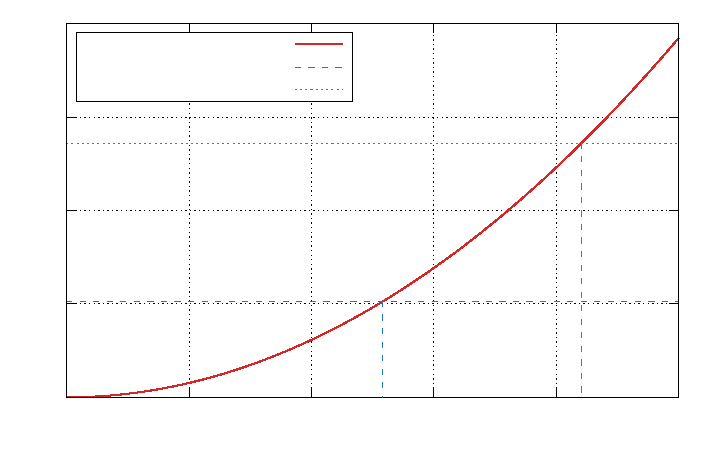
\includegraphics[width={340.00bp},height={226.00bp}]{images/physik/luftwiderstand}}%
    \gplfronttext
  \end{picture}%
\endgroup

    \caption{Der Luftwiderstand...}
    \label{fig:physik:bewegung:luftwiderstand}
\end{figure}


